%%%%%%%%%%%%%%%%%%%%%%%%%%%%%%%%%%%%%%%%%%%%%%%%%%%%%%%%%%%%%%%%%%%%%%
%%                           INTRODUCTION
%%%%%%%%%%%%%%%%%%%%%%%%%%%%%%%%%%%%%%%%%%%%%%%%%%%%%%%%%%%%%%%%%%%%%


\pagestyle{plain} % No headers, just page numbers
\pagenumbering{arabic} % Arabic numerals
\setcounter{page}{1}


\chapter{Introduction}
The rapid internet adoption in everyday life and the workplace has presented us with new security challenges. Users are more active on the internet, giving attackers more opportunities to attack unsuspecting victims. There are various technical security measures such as firewall, encryption, threat hunting software, and engaging automation to mitigate these challenges. However, studies have shown that the human layer is the weakest link in the security chain \cite{jampen} and attackers usually start by targeting the most vulnerable link before performing other detrimental attacks. These attacks with human interaction are generally known as "Social Engineering Attacks" and use psychological manipulation to trick users into making security mistakes or giving away sensitive information.

\section{What is phishing?}
Phishing is an example of social engineering attack in which attackers target users by contacting them through email, telephone, or text message by someone posing as a legitimate \cite{phishing, apwg}. These attacks are challenging to detect as attackers use the computing infrastructure to fool the victim into doing something but are doing something else while the computing system is working as intended. Due to this, even users with a high-end security system can be victims. An example of such is the infamous case of John Podesta \cite{podesta}, Hilary Clinton's campaign chairman for the 2016 presidential election. The "googlemail.com" in the domain successfully tricked John Podesta and the Clinton campaign's computer help desk to trust the email(See fig:\ref{fig:Podesta}).

\begin{figure}[ht]
    \centering
    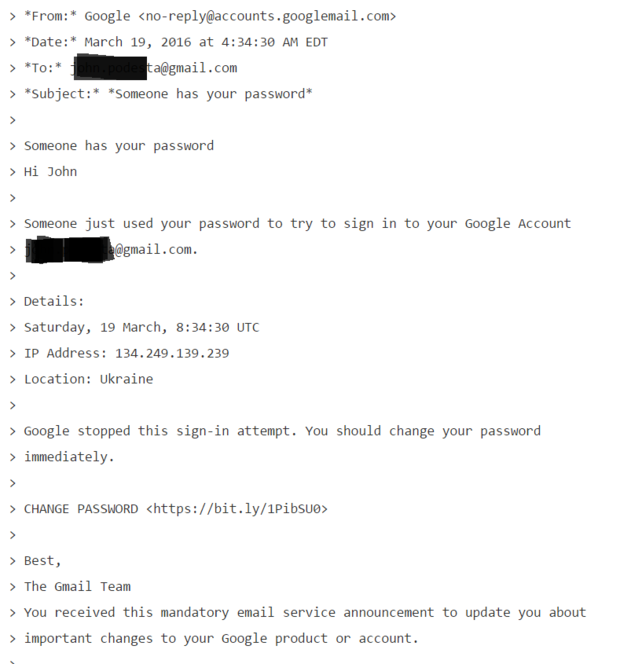
\includegraphics[scale=0.7]{{./podesta.png}}
    \caption[Phishing email sent to John Podesta]{Phishing email sent to John Podesta}
    \label{fig:Podesta}
\end{figure}

Successful phishing attacks can be costly to an organization. For example, in 2020, attacks cost US businesses more than \$1.8 billion, up from \$1.7 billion in 2019 \cite{vade}. In addition, these attacks can also lead to credential/account compromise leading to leaks of sensitive information. In 2014, an attack was successful on an invasion of celebrity iCloud accounts, leading to the embarrassing leaking of nude photos. The leak was initially considered due to a breach on Apple services, but it was later a phishing attack pretending to be Apple and Google and asking them to change their password \cite{duke_2014, guardian_2014}.

Phishing attacks have been continuously rising and have doubled since early 2020. In July 2021 alone, APWG saw 260,642 phishing attacks \cite{apwg}. Additionally, Proofpoint found that more than 75\% of organizations faced phishing attacks in 2021 \cite{proofpoint}. These uprising trends in attacks have shown some serious need for mitigations for phishing attacks.

\section{Current Mitigations}
The prevention of phishing attacks can be divided into three steps \cite{vayansky}. The first step to stop a phishing attack is preventing the attack from reaching the end-user. We have seen multiple studies on phishing prevention with the help of the machine learning approach \cite{yang_zheng_wu_wu_wang_2021, sahingoz_buber_demir_diri_2019}. Although these models may catch some sites, it is impossible to filter out and prevent phishing attacks. The phisher can easily make a new site and learn to create better contextual attacks, preventing these models from being fully effective.

It is impossible to stop all the attacks as attackers usually design their attacks to reach vulnerable users. However, many web browsers and email clients are already prepared to warn users of any suspicious activities they detect. For example, browsers use active warnings such as "This page is not secure warnings" to warn the users of any certificates they fail to verify or pop up windows with a sign that the site they are on is suspected of forgery. In addition, there are other passive indicators, such as different shades of link highlights in the address bar, security lock signs, etc., that browsers use. Active warnings prevent more attacks \cite{vayansky}, but attackers can easily bypass these warnings by creating new sites and new contextual websites.

\begin{figure}[h]
    \centering
    
\includegraphics[scale=0.7]{{./browser_cues.png}}
    \caption[Browser cues on links]{Browsers uses different shades to indicate the primary link and the secondary links.}
    \label{fig:browser_cues}
\end{figure}

The final step to avoid phishing emails is user training. A study done by Proofpoint shows that 34\% of US respondents believe emails with familiar logos are safe \cite{proofpoint}. The study indicates a general lack of awareness about phishing campaigns among the general population. There are many tools used for phishing training. One of the most common tools to train users is cyber security videos. However, a study shows that these videos are only efficient only if the user pays attention through all of them \cite{what_hack}. We can also find other techniques such as reading materials and cyber security classes to raise awareness among users.

Although these training help users recognize phishing attacks, simply knowing does not provide helpful strategies for identifying phishing attacks. In addition, the lack of contextual information in these videos leaves room for improvement. Therefore, an interactive user program that conveys the information with a better approach is necessary. Our approach to using the game to spread awareness tries to tackle this problem.

\section{Litearature Review}
The gaming approach to train users is not novel. Hendrix et al. \cite{hendrix_al_sherbaz_bloom_2016} investigated whether games can be effective cyber security training tools with some of the popular games designed for cyber security training. Their study indicated positive signs, although there was insufficient evidence to draw definite conclusions.

\subsection{Educational Games}
\subsection{Board Game}
ctrlalthack

smells phishy

\subsection{Phishing Link training}
antiphishing phil

phish phinder - same as antiphishing phil

gamified approach - shooting game


\subsection{Role playing game}
what dot hack

\section{Objective}